\documentclass[12pt, twoside]{article}
\usepackage[letterpaper, margin=1in, headsep=0.5in]{geometry}
\usepackage[english]{babel}
\usepackage[utf8]{inputenc}
\usepackage{amsmath}
\usepackage{amsfonts}
\usepackage{amssymb}
\usepackage{tikz}
%\usetikzlibrary{quotes, angles}

\usepackage{graphicx}
\usepackage{enumitem}
\usepackage{multicol}

\usepackage{fancyhdr}
\pagestyle{fancy}
\fancyhf{}
\renewcommand{\headrulewidth}{0pt} % disable the underline of the header

\fancyhead[LE]{\thepage}
\fancyhead[RO]{\thepage \\ Name: \hspace{4cm} \,\\}
\fancyhead[LO]{BECA / Dr. Huson / Geometry\\* Unit 7: Similarity\\* 13 January 2020}

\begin{document}
\subsubsection*{7.9 Classwork: Constructions}
  \begin{enumerate}

  \item Complete the construction of a perpendicular bisector of $\overline{AB}$. Label the midpoint $M$. Show all construction marks, but make no extra lines. \vspace{2cm}
    \begin{center}
    \begin{tikzpicture}
      \draw [-, thick] (0,0)--(4,5);
      \draw [fill] (0,0) circle [radius=0.05] node[below right]{$A$};
      \draw [fill] (4,5) circle [radius=0.05] node[above left]{$B$};
    \end{tikzpicture}
    \end{center} \vspace{4cm}

  \item Accurately draw a square that is 5 centimeters on each side.

\newpage
  \item Complete the construction of an equilateral triangle with one side as $\overline{XY}$. Show all construction marks, but make no extra lines. \vspace{3cm}
  \begin{center}
  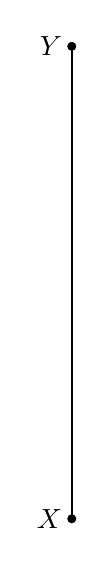
\begin{tikzpicture}
    \draw [-, thick] (0,0)--(0,6);
    \draw [fill] (0,0) circle [radius=0.05] node[left]{$X$};
    \draw [fill] (0,6) circle [radius=0.05] node[left]{$Y$};
  \end{tikzpicture}
  \end{center} \vspace{3cm}
  \begin{enumerate}
    \item Identify two circles in the construction. For each, name the center of the circle and the radius.  \vspace{3cm}
    \item Assuming that the third vertex of the triangle is point $Z$, explain why the distance from $X$ to $Z$ is the same as the distance from $X$ to $Y$.
  \end{enumerate}

\newpage
  \item Complete the construction of a line perpendicular to line $l$ through the point $P$. Show all construction marks, but make no extra lines. \vspace{3cm}
  \begin{center}
  \begin{tikzpicture}
    \draw [<->, thick] (-5,0)--(7,0)node[below]{$l$}--(8,0);
    \draw [fill] (3,3) circle [radius=0.05] node[above left]{$P$};
  \end{tikzpicture}
  \end{center} \vspace{7cm}

  \item The perimeter of a square is 52 cm. Find the area of the square.


\end{enumerate}
\end{document}